\label{subsec:precision_timing_inst_ptarm}
Worst-case execution time (WCET) analysis requires a combination of software analysis to determine the worst-case path, and architectural analysis to determine the time it takes to execute that paths on the underlying architecture. 
A plethora of research has been done on the software analysis of program paths. 
Wilhelm et al.~\cite{wilhelm-survey-paper} present a survey of tools and techniques available for worst-case path enumeration, loop analysis, etc.
However, the precision of the WCET analysis of those techniques ultimately depends on the underlying architecture implementation~\cite{Heckmann2003processor}.
Architectures that exhibit wildly unpredictable execution times will result in overly conservative WCET analysis, even if the software structure is simple. 
Designed as a predictable architecture, the instructions of PTARM all exhibit deterministic timing behaviors, allowing precise architectural analysis for the WCET analysis.
Table~\ref{table:ptarm_instruction_timing} summarizes the execution time each instruction takes in terms of \emph{thread cycles}. 

\begin{table}[h]
\vspace{-5pt}
\noindent\makebox[\textwidth]{%
\begin{smalltabular}{  l  c || l | c | c | }
  \cline{4-5}                        
  \multicolumn{3}{l|}{}  & \multicolumn{2}{|c|}{\textbf{Memory Region Accessed}}   \\ \hline 
  \multicolumn{1}{|l|}{\textbf{Instruction}} & \multicolumn{1}{|c||}{\textbf{Latency}} & \textbf{Instruction (\emph{\scriptsize{Addressing Mode}})} & \textbf{SPM/Boot}  & \textbf{DRAM}   \\ \hline \hline
  \multicolumn{1}{|l|}{Data Processing}  & \multicolumn{1}{|c||}{1} & 
  \multicolumn{1}{|l|}{Load Register (\emph{\scriptsize{offset}})}  & 1 & 4$^{\phi}$ \\ \hline
  \multicolumn{1}{|l|}{Branch}  & \multicolumn{1}{|c||}{1} &
  \multicolumn{1}{|l|}{Load Register (\emph{\scriptsize{pre/post-indexed}})}  & 2 & 5$^{\phi}$ \\ \hline
  \multicolumn{1}{|l|}{Software Interrupt (SWI)}  & \multicolumn{1}{|c||}{1} &
  \multicolumn{1}{|l|}{Store Register (\emph{\scriptsize{all}})} & 1 & 2$^{\delta}$ \\ \hline
  \multicolumn{1}{|l|}{get\_time}  & \multicolumn{1}{|c||}{2}  &
  \multicolumn{1}{|l|}{Load Multiple (\emph{\scriptsize{offset}})} & $N_{reg}$ & $N_{reg}\times 4^{\phi}$ \\ \hline
  \multicolumn{1}{|l|}{delay\_until}  & \multicolumn{1}{|c||}{1$^{\dagger}$} &
  \multicolumn{1}{|l|}{Load Multiple (\emph{\scriptsize{pre/post-indexed}})} & $N_{reg} + 1$  & $(N_{reg}\times 4^{\phi})+1$  \\ \hline
  \multicolumn{1}{|l|}{exception\_on\_expire}  & \multicolumn{1}{|c||}{1} &
  \multicolumn{1}{|l|}{Store Multiple (\emph{\scriptsize{all}})}  & $N_{reg}$ & $N_{reg}\times 2$  \\ \hline
  \multicolumn{1}{|l|}{deactivate\_exception}  & \multicolumn{1}{|c||}{1} &
   &  &   \\ \hline
  \multicolumn{5}{|l|}{\textbf{Notes:}} \\ \hline
  \multicolumn{5}{|p{.9\textwidth}|}{\scriptsize{$N_{reg}$: This is number of registers in the register list.}} \\
  \multicolumn{5}{|p{.9\textwidth}|}{\scriptsize{$^{\delta}$: The single store buffer (described in section~\ref{sec:ptarm_dram_store_buffer}) can hide the store latency to DRAM, making it 1 thread cycle. But in cases where the store buffer cannot be used, the latency is 2 thread cycles.}} \\
  \multicolumn{5}{|p{.9\textwidth}|}{\scriptsize{$^{\phi}$: The DRAM load latency is 3 or 4 thread cycles depending on the alignment of the pipeline and the DRAM controller backend, as described in section~\ref{sec:ptarm_dram_integration}. For conservative estimates, 4 thread cycles is used.}} \\
  \multicolumn{5}{|p{.9\textwidth}|}{\scriptsize{$^{\dagger}$: This is the minimum execution time of \delayuntil. The actual execution time varies depending on the input timestamp.}} \\ \hline
\end{smalltabular}}
\vspace{1mm}
\caption{Timing properties of PTARM instructions (in thread cycles)}
\label{table:ptarm_instruction_timing}
\end{table}

\newcommand{\e}[1]{\ensuremath{\times 10^{#1}}}

A \emph{Thread cycle} is the unit used to represent execution time for each thread.  
Timing analysis can be done separately for each hardware thread running on PTARM because the threads are temporally isolated; the execution time of each thread is not affected by other threads.
The thread-interleaved pipeline switches thread contexts every processor cycle in a predictable round robin fashion. 
Thus, each thread is fetched and executed in the pipeline every $N$ processor cycles, $N$ being the number of threads in the pipeline.
One \emph{Thread cycle} represents each time the thread enters in the pipeline, which is the thread's perceived notion of cycles.
The execution frequency of each thread ($F_{thread}$) is $F_{processor}/N$, so each \emph{thread cycle} is $1/F_{thread}$ long. 
Our PTARM core is clocked at 100$MHz$ ($F_{processor} = 100\e{6}$) and has 4 threads ($N=4$) , so each thread cycle is $\frac{1}{(100\e{6})/4} = 40\e{-9}$ secs, or $40ns$ long.
The length of the \emph{thread cycle} will not change because of the predictable thread-switching policy, making it a reliable unit of measurement for execution time.   

\subsection{Memory instructions}
Data-processing and branch instructions have straightforward execution times.
The execution time of branches is deterministic because the branch penalty is completely hidden by the thread interleaving.
On the other hand, memory instructions in our architecture can have several different latencies depending on addressing mode or region of access, as listed in table~\ref{table:ptarm_instruction_timing}.
For memory instructions that use pre or post-indexed addressing mode to update the base register, an additional cycle latency is needed to write back to the base register.
This is documented in the instruction implementation of load/store register in section~\ref{sec:ptarm_instruction_ldstr}.
The addressing mode of load/store instructions is specified as part of the instruction binary.
Thus, it can be determined statically and does not affect the complexity or precision of execution time analysis. 

Different memory technologies provide different access latencies. 
The exposed memory hierarchy allows us to clearly label and identify access latencies based on the address accessed by the memory instruction.
In execution time analysis tools, \emph{value analysis} attempts to determine the address accessed by each instruction~\cite{wilhelm-survey-paper}.
Once the \emph{value analysis} determines the memory address, a precise memory access latency can be associated with the memory instruction.    
This allows for a simpler timing analysis and more accurate execution analysis compared to conventional memory hierarchies with caches. 
If caches are used to hide the memory hierarchy, additional modeling of the cache state is required after the \emph{value analysis} to predict the cache state and determine whether the access hit or misses the cache. 

For store instructions, the single store buffer described in section~\ref{sec:ptarm_dram_store_buffer} can usually hide the latency to access DRAM, if the subsequent instruction does not access the DRAM. 
Otherwise the store to DRAM will observe full memory access latency of two thread cycles.
Architectural timing analysis can account for the store buffer by statically checking the next instruction to see whether it is a memory accessing instruction to the DRAM.
Since only one instruction needs to be checked, it only slightly complicates the timing analysis.
If it is not possible, then the full store to DRAM latency can be used for conservative analysis. 

The execution time of load/store multiple instructions depend on the number of registers operated on, and the memory region it accesses. 
Because the register list is statically encoded in the instruction, the number of registers operated on can be determined statically.
For each register that is operated on, the latency will depend on which memory region it accesses. 
The total execution time of the instruction will be the sum of the latencies for all register operations. 
Store multiple instructions to the DRAM do not benefit from the store buffer, because they issue consecutive stores to the DRAM. 
Thus, each store takes the full DRAM store latency.
If pre or post-indexed addressing mode is used, an extra cycle is added to update the base register, just as regular load/store instructions. 

\subsection{Timing instructions}
\label{sec:jitter_of_timing_instructions}
With the exception of \delayuntil, which by design exhibits variable execution time, the execution time of all other timing instructions is static.  
However, the timing instructions can impact the execution time of the program in a very dynamic way.
For example, the execution of \exceptiononexpire\ and \deactivateexception\ only take one thread cycle, but when the \timerexpired\ exception is thrown, the execution time of the whole program dynamically changes. 
To precisely understand the timing effects of the timing instructions, we must understand the jitter of the timing instructions caused by the underlying implementation.
It is impossible for any hardware implementation to provide absolute precision of time, as we are limited by the digital synchronous circuits that discretize the notion of time. 
Although the timing extensions allow the manipulation of timestamps, representing nanoseconds, in software, with the thread-interleaved pipeline in PTARM, the basic unit of time for each thread is one thread cycle, or $40ns$.
In other words, $40ns$ is the shortest interval of time that is observable by each thread.
This can also be understood from the implementation of the thread-interleaved pipeline.
Each thread only latches the clock value in the fetch stage, and the timestamp is propagated along the pipeline and associated with the instruction. 
Since there are four threads cycling in a round robin fashion, each thread latches the clock value only once every 4 processor cycles. 
With 100MHz clocking the pipeline in our implementation, 4 processor cycles is equivalent to $40ns$.

When manipulating timestamps, the execution time of the timing instructions and jitter must be accounted for.
The timestamp associated with each instruction represents the \emph{time of execution} of that instruction.
In our implementation, the \emph{time of execution} is when the instruction begins to execute, so the timestamp is latched in the fetch stage.
This is the value stored into registers for \gettime\ instructions.  
%This means the timestamp obtained from \gettime\ will contain the time at the beginning of execution of \gettime.
Since \gettime\ takes 2 thread cycles to complete, $80ns$  will have elapsed when the next instruction begins its execution.
In the same way, \delayuntil\ delays programs execution until the current \emph{time of execution} is greater than or equal to the input timestamp value.
When \delayuntil\ completes its execution, the next instruction will observe a platform time of \emph{at least} $40ns$ greater than the input timestamp passed to \delayuntil.
This effect is illustrated in figure~\ref{fig:delay_until_details}.
\begin{figure}[h]
  \begin{center}
    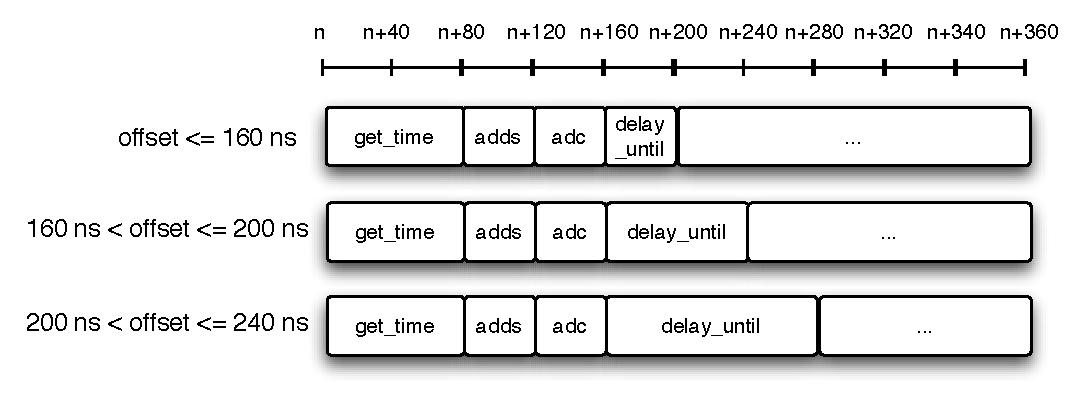
\includegraphics[scale=.7]{figs/delay_until_details}
  \end{center}
  \vspace{-3mm}
  \caption{Timing details of get\_time and delay\_until}
  \label{fig:delay_until_details}
\end{figure}

The code segment starts executing at time $t$. 
The code only consists of \gettime, \delayuntil, and 2 add instructions used to add an offset to the timestamp obtained by \gettime.
In all 3 cases, the timestamp obtained by \gettime\ would contain the value $t$, and the instruction after \gettime\ executes at $t+80$.
Taking into account the 2 thread cycles used to add the offset to the timestamp, if the offset is $\leq 160$, then the \delayuntil\ will simply serve as a NOP. 
This is because when \delayuntil\ is executed, it will latch $t+160$ for the current time, and it will only delay program execution if the input timestamp is $> t+160$.
This is the top case shown in the figure.
The instruction after \delayuntil\ executes at time $t+200$, which accounts for the 1 thread cycle it takes to execute \delayuntil.
Assuming \delayuntil\ does delay the program, in the worst-case, the instruction after \delayuntil\ can execute $79 ns$ after the input timestamp. 
This can be observed if the offset is set to 161, which is shown in the middle timeline in figure~\ref{fig:delay_until_details}.  
\Delayuntil\ will first latch the time $t+160$ to compare with the input timestamp of $t+161$. 
Because current platform time is less than the input timestamp, even by $1ns$, \delayuntil\ will delay the execution of the program until the next cycle, when $t+200$ is latched to be compared against the input timestamp. 
At that point, \delayuntil\ will complete its execution, and the next instruction will execute at $t+240$.
This jitter results from the minimum observable time interval of $40 ns$ for each thread, causing \delayuntil\ to have an observable jitter of up to $39 ns$. 

For each thread, the hardware \emph{timer} unit checks an activated deadline slot once every thread cycle ($40ns$). 
Thus, the triggering of \timerexpired\ exceptions from the \emph{timer} unit also observes a similar jitter effect. 
This is illustrated in figure~\ref{fig:timing_exception_details}.  
\begin{figure}[h]
  \begin{center}
    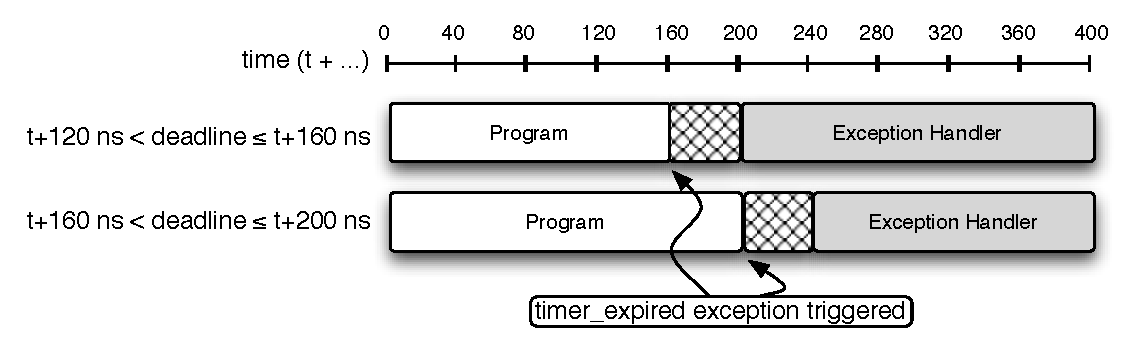
\includegraphics[scale=.7]{figs/timing_exception_details}
  \end{center}
  \vspace{-3mm}
  \caption{Timing details of the \timerexpired\ exception triggering}
  \label{fig:timing_exception_details}
\end{figure}
If the thread has a deadline of $t+161ns$, then the actual exception will not be triggered until $t+200ns$, when the observed platform time is greater than the deadline. 

\subsection{Timed Loop revisited}
\label{sec:timed_loop_revisited}
We give a concrete example of analysis of timing instructions on PTARM by deriving the \emph{offset} from the self compensating timed loop introduced in section~\ref{sec:timed_loops}.
This timed loop detects whether the previous loop iteration missed its deadline. 
If it did, then the current iteration will execute a shorter version of the task in attempt to make up for the lost time, as shown in figure~\ref{fig:self_compensating_loop_timing}.  
\begin{figure}[h]
  \vspace{-3mm}
  \begin{center}
    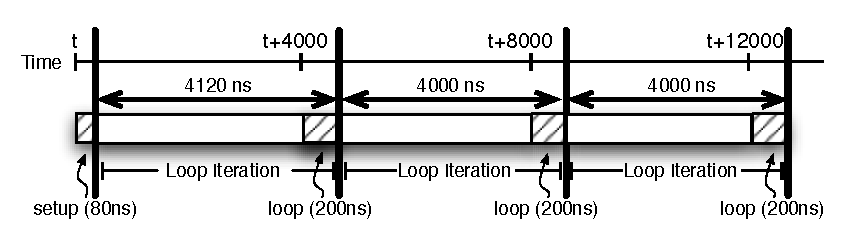
\includegraphics[scale=.7]{figs/self_compensating_loop_timing}
  \end{center}
  \vspace{-3mm}
  \caption{Execution of the self compensating timed loop}
  \label{fig:self_compensating_loop_timing}
\end{figure}
\vspace{-8mm}
\begin{lstlisting}[float=h, label=lst:timed_loop_compensate_revisit,caption=Timed loops with compensation revisited]
  cdp p13, 8, c2, c0, c0, 0  ; get_time, deadline timestamp stored in [c2, c3]
loop:
  cdp p13, 8, c4, c0, c0, 0  ; get_time, current timestamp stored in [c4, c5]
  subs r5, r5, #80           ; compensate for loop overhead and delay_until 
  sbc  r4, r4, #0            ; 

  subs r5, r3, r5            ; Check whether previous iteration deadline is missed
  sbc  r4, r2, r4            ; 

  blmi task_short            ; execute shorter task if previous deadline miss 
  blpl task_normal           ; or else execute normal task 
  
  adds r3, r3, #4000         ; assuming the deadline is 4 us (4000 ns)
  adc r2, r2, #0             ; calculate the deadline timestamp for this iteration
  cdp p13, 4, c2, c2, c3, 0  ; delay_until
   
  b loop
\end{lstlisting}

\subsubsection{Obtaining the offset}
Listing~\ref{lst:timed_loop_compensate_revisit} shows the source code that is used to construct this timed loop. 
During the miss detection (lines 3 to 8), an additional \textit{offset} is used to compensate for the execution of \delayuntil\ and loop overhead.
Time elapses between the \delayuntil\ of the previous loop iteration (line 15), where the previous deadline timestamp is checked, and the \gettime\ is used for miss detection (line 3) in the current iteration.
Without the offset compensation, the loop overhead will cause the miss detection to always detect a missed deadline.
This can be observed from table~\ref{table:timed-loop-compensate-timing}, where we show a sample execution trace of four iterations in this timed loop.  
Figure~\ref{fig:self_compensating_loop_timing} shows the timing behavior of these four iterations, where a missed deadline in the second iteration will cause the third iteration to compensate by executing the shorter version of the task.

\begin{table}
\vspace{-5mm}
\begin{center}
\noindent\makebox[\textwidth]{%
\begin{smalltabular}{ | l | l | l r | }
  \hline
  \textbf{Time} & \textbf{TC} & \textbf{Instruction} & \textbf{Comment}\\ \hline \hline 
  t ns & n &  \textit{cdp p13, 8, c2, c0, c0, 0} & get\_time (deadline: t) \\  \hline
  \multicolumn{4}{|c|}{ -- -- Loop 1st iteration / No deadline miss -- -- } \\ \hline    
  t+80 ns & n+2 &  \textit{cdp p13, 8, c4, c0, c0, 0 } & get\_time, (current: t+80) \\
  t+160 ns & n+4 &  \textit{subs r5, r5, \#80} & (current -= 80)\\
  t+200 ns & n+5 &  \textit{sbc  r2, r2, r4} & (current: t)\\  
  t+240 ns & n+6 &  \textit{subs r5, r3, r5} & compare deadline (t) and current (t) \\
  t+280 ns & n+7 &  \textit{sbc  r4, r2, r4} & result is 0, clear cc[``n''] \\
  t+320 ns & n+8 &  \textit{blmi task\_short} & nop since cc[``n''] == 0\\
  t+360 ns & n+9 &   \textit{blpl task\_normal} & branch since cc[``n"] == 0\\  
    - ns & - &  \ldots & executing task\_normal \\  
  t+3800 ns & n+95 & \textit{adds r3, r3, \#4000} &  (deadline += 4000) \\
  t+3840 ns & n+96 & \textit{adc r2, r2, \#0} &  (deadline: t+4000) \\ 
  t+3880 ns & n+97 &  \textit{cdp p13, 4, c2, c2, c3, 0} & delay\_until, input timestamp is t+4000\\
  - ns & - & \ldots & delay\_until for 3 thread cycles\\  
  t+4040 ns & n+101 &  \textit{b loop} & jump back to loop \\ \hline
  \multicolumn{4}{|c|}{ -- -- Loop 2nd iteration / Deadline miss -- -- } \\ \hline    
  t+4080 ns & n+102 &  \textit{cdp p13, 8, c4, c0, c0, 0 } & get\_time, (current: t+4080)\\
  t+4160 ns & n+104 &  \textit{subs r5, r5, \#80} & (current -= 80)\\
  t+4200 ns & n+105 &  \textit{sbc  r2, r2, r4} & (current: t+4000)\\  
  t+4240 ns & n+106 &  \textit{subs r5, r3, r5} & compare deadline (t+4000) and current (t+4000)\\
  t+4280 ns & n+107 &  \textit{sbc  r4, r2, r4} & result is 0, clear cc[``n''] \\
  t+4320 ns & n+108 &  \textit{blmi task\_short} & nop since cc[``n''] == 0\\
  t+4360 ns & n+109 &   \textit{blpl task\_normal} & branch since cc[``n"] == 0\\  
  - ns & - &  \ldots & code for task\_normal \\  
  t+7960 ns & n+199 & \textit{adds r3, r3, \#4000} & (deadline += 4000) \\
  t+8000 ns & n+200 & \textit{adc r2, r2, \#0} & (deadline: t+8000) \\ 
  t+8040 ns & n+201 &  \textit{cdp p13, 4, c2, c2, c3, 0} & delay\_until, *no delay*\\
  t+8080 ns & n+202 &  \textit{b loop} & jump back to loop \\ \hline
  \multicolumn{4}{|c|}{ -- -- Loop 3rd iteration / Compensate with shorter task -- -- } \\ \hline    
  t+8120 ns & n+203 &  \textit{cdp p13, 8, c4, c0, c0, 0 } & get\_time, (current: t+8120)\\
  t+8200 ns & n+205 &  \textit{subs r3, r3, r5} & (current -= 80)\\
  t+8240 ns & n+206 &  \textit{sbc  r2, r2, r4} & (current: t+8040) \\
  t+8280 ns & n+207 &  \textit{subs r5, r3, r5} & compare deadline (t+8000) and current (t+8040)\\
  t+8320 ns & n+208 &  \textit{sbc  r4, r2, r4} & result is -40, set cc[``n''] \\
  t+8360 ns & n+209 &  \textit{blmi task\_short} & branch since cc[``n"] == 1 \\
  - ns & - &  \ldots & code for task\_short \\  
  t+10280 ns & n+257 &   \textit{blpl task\_normal} & nop since cc[``n''] == 1\\    
  t+10320 ns & n+258 & \textit{adds r3, r3, \#4000} & (deadline += 4000) \\
  t+10360 ns & n+259 & \textit{adc r2, r2, \#0} & (deadline: t+12000) \\ 
  t+10400 ns & n+260 &  \textit{cdp p13, 4, c2, c2, c3, 0} & delay\_until\\
  - ns & - &  \ldots & delay until time is t+12000 \\  
  t+12040 ns & n+301 &  \textit{b loop} & jump back to loop \\ \hline
   \multicolumn{4}{|c|}{ -- -- Loop 4th iteration / Execute normal task -- -- } \\ \hline    
  t+12080 ns & n+302 &  \textit{cdp p13, 8, c4, c0, c0, 0 } & get\_time, (current: t+12080)\\
  t+12160 ns & n+304 &  \textit{subs r3, r3, r5} & (current -= 80)\\
  t+12200 ns & n+305 &  \textit{sbc  r2, r2, r4} & (current: t+12000) \\
  t+12240 ns & n+306 &  \textit{subs r5, r3, r5} & compare deadline (t+12000) and current (t+12000)\\
  t+12280 ns & n+307 &  \textit{sbc  r4, r2, r4} & result is 0, clear cc[``n''] \\
  \hline 
\end{smalltabular}}
\end{center}
\vspace{-3mm}
\caption{Instruction execution trace of the self compensating timed loop\\ (TC = thread cycles)}
\label{table:timed-loop-compensate-timing}
\end{table}

In table~\ref{table:timed-loop-compensate-timing}, execution starts at time $t$.
As mentioned before, each thread cycle is $40ns$, which is reflect in the left most column that shows the progression of time.
We also show the thread cycle (TC) count, which starts at $n$ when execution begins.
The execution time of each instruction is according to table~\ref{table:ptarm_instruction_timing}.
All instructions are statically compiled onto the instruction scratchpad.
In this code segment, we keep track of two timestamps each iteration. 
The \emph{deadline\_timestamp} keeps track of the loop deadlines, and is stored in registers r2 and r3.  
The \emph{current\_timestamp} is updated with \gettime\ in the beginning of each loop iteration to detect if the previous iteration missed its deadline.
It is stored in registers r4 and r5. 
The loop period is set to be $4 \mu s$, which is $4000 ns$ (100 thread cycles).
We add the loop period to the \emph{deadline\_timestamp} in each loop iteration (lines 13 and 14).  

\newcommand{\currentt}{\emph{current\_timestamp}}
\newcommand{\deadlinet}{\emph{deadline\_timestamp}}


The need for the \emph{offset} can be observed at the beginning of the second loop iteration.
At time $t+4080ns$, \gettime\ is called to initiate the miss detection sequence.
The previous \deadlinet\ is $t+4000$, which was met in the first iteration.  
However, \gettime\ updates the \currentt\ to $t+4080$, because the execution of \delayuntil\ and \emph{b loop} took 2 thread cycles combined. 
Thus, our miss detection needs to account for this by subtracting the 2 thread cycles ($80ns$) difference from \currentt\ before comparing it with \deadlinet.
In general, the \emph{offset} that needs to be accounted for is the time elapsed between the deadline checking \delayuntil\ instruction and the miss detection \gettime\ instruction.
Intuitively, we want to check whether the previous \delayuntil\ executed before the previous \deadlinet, so the \emph{offset} is calculates the time of execution of the previous \delayuntil.  

\subsubsection{Overhead of the self compensating timed loop}
In this self compensating timed loop, the loop period is set to $4000ns$ and regulated with the \delayuntil\ instruction.
Each loop period includes the execution of the actual task along with the loop and timing control overhead.
The loop overhead in this example is only the branch instruction on line 17 in listing~\ref{lst:timed_loop_compensate_revisit}, which is 1 thread cycle (40 ns).
The overhead for timing control and self compensation consists of all the timing instructions, the arithmetic on the timestamps, and the 2 conditional branch instructions that determine which task to execute.
From table~\ref{table:timed-loop-compensate-timing} we can count a total overhead of 11 thread cycles which includes: 1 \gettime\ (2 thread cycles), 1 \delayuntil\ (1 thread cycle), 6 arithmetic operations on the timestamps (6 thread cycles), and 2 conditional branch instructions (2 thread cycles).
Overall the timed loop contains an overhead of 12 thread cycles ($480ns$) , which means both tasks have a soft timing requirement of 88 thread cycles ($3520ns$) for each loop iteration to meet its deadline.  
In the second loop iteration of our example, \emph{task\_normal} executes for 89 thread cycles, exactly one thread cycle over its timing requirement. 
As a result, the \delayuntil\ of the second loop iteration does not delay program execution, and the third iteration miss detection detects a missed deadline and switches to execute \emph{task\_short}. 

\subsubsection{First loop iteration jitter}
The \emph{offset} previously derived is the time difference between the desired deadline and the time of execution of the \gettime\ used for miss detection.  
In our code, because of the simple loop structure, the \emph{offset} only includes the execution time of the \delayuntil\ and a branch. 
However, if the difference was larger, for example, in a conditional loop structure, then it could introduce jitter for the first iteration.
An example is shown in figure~\ref{fig:setup_look_timing}.
\begin{figure}[h]
  \vspace{-3mm}
  \begin{center}
    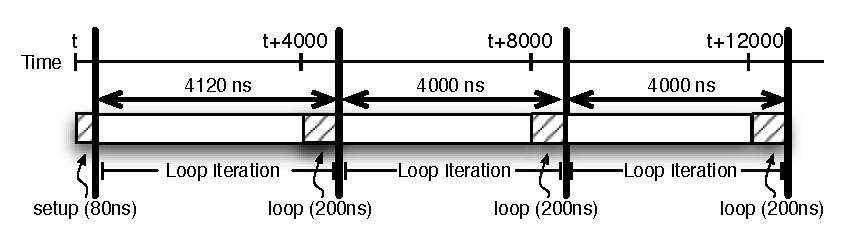
\includegraphics[scale=.9]{figs/setup_loop_timing}
  \end{center}
  \vspace{-3mm}
  \caption{Jitter caused by initial timed loop setup}
  \label{fig:setup_look_timing}
\end{figure}
We assume that the setup code remains the same with only one \gettime, and the \emph{offset} is adjusted to 200ns.
We also assume that the loop period remains the same, 4000ns, and all loop iterations meet the loop period timing requirements. 
In this example, we see that the first iteration executes for 120ns longer than subsequent iterations.
The jitter introduced for the first iteration is exactly the execution time difference between the \emph{offset} and the setup code.  
Between each \delayuntil\ instruction, exactly 4000 ns elapses, since 4000 ns is used as the loop period and added to the \deadlinet\ each loop iteration.   
From the figure we observe that the execution of \emph{offset} occurs between each subsequent \delayuntil\ instruction.
However, between the initial \deadlinet\ value ($t$) and the first \delayuntil, the only overhead that is observed is the execution of a \gettime\ instruction, which is 80 ns. 
Thus, the first iteration of the loop executes for an addition $120ns$, which is the difference between the \emph{offset} and the execution time of the loop setup code.
This effect is not observed in the previous example because the execution time of both \emph{offset} and loop setup is $80 ns$, so the first iteration also executed for exactly 4000 ns.   

\begin{lstlisting}[float=h, label=lst:timed_loop_compensate_adj,caption=Jitter adjusted timed loop ]
  mov r6, #0                 ; i = 0;
  mov r7, #0                 ; j = 0;
  
  cdp p13, 8, c2, c0, c0, 0  ; get_time, deadline timestamp stored in [c2, c3]
  subs r3, r3, #40           ; adjustment for first loop period 
  sbc  r2, r2, #0            ; deadline -= 40
loop:
  cdp p13, 8, c4, c0, c0, 0  ; get_time, current timestamp stored in [c4, c5]
  subs r5, r5, #200          ; compensate for loop overhead and delay_until 
  sbc  r4, r4, #0            ; 

  subs r4, r3, r5            ; Check if previous iteration deadline is missed
  sbc  r5, r2, r4            ; 

  blmi task_short            ; execute shorter task if previous deadline mess 
  blpl task_normal           ; or else execute normal task 
  
  adds r3, r3, #4000         ; assuming the deadline is 4 us (4000 ns)
  adc r2, r2, #0             ; calculate the deadline timestamp for this iter.
  cdp p13, 4, c2, c2, c3, 0  ; delay_until
	
  add r6, r6, #1             ; i += 1    
  add r7, r7, r6 LSL #1      ; j += i*2  
  cmp r7, #1000              ; 
  blt loop                   ; branch back if ( j < 10000 )
\end{lstlisting} 

\begin{figure}[h]
  \vspace{-3mm}
  \begin{center}
    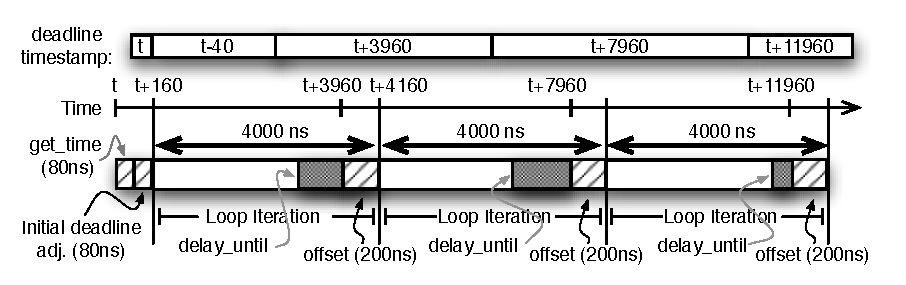
\includegraphics[scale=.9]{figs/setup_loop_timing_adj}
  \end{center}
  \vspace{-3mm}
  \caption{Adjusted timed loop setup}
  \label{fig:setup_look_timing_adj}
\end{figure}

This first iteration jitter can be accounted for by adjusting the initial \deadlinet\ in the loop setup code.
In listing~\ref{lst:timed_loop_compensate_adj} we show the source code that adjusts for the initial loop iteration jitter.
Lines 22 to 25 show the additional loop overhead that conditionally checks whether to branch back to the beginning of the loop.
The \emph{offset} that we have to adjust for in this example is exactly 200ns, which includes the 4 instructions for the loop overhead and the \delayuntil. 
This offset is accounted for on line 9.
Lines 4 to 6 show the loop setup code where we adjust for the execution time of the initial loop iteration.
40 is subtracted from the initial \deadlinet\ obtained by the \gettime\ on line 4.
This value is obtained by the execution time difference of the \emph{offset} ($200ns$) and the setup code ($160ns$).
We show the resulting timing behavior in figure~\ref{fig:setup_look_timing_adj}, where the first loop iteration is adjusted to 4000ns, the same as subsequent iterations.
By entering the loop with the \deadlinet\ value of $t-40$, we shift the \delayuntil\ deadlines for all loop iterations by 40 ns, which compensates for the initial loop iteration jitter.   
Intuitively, the initial \deadlinet\ is adjusted before the loop to create the illusion that the setup code and the loop overhead observed between each \delayuntil\ has the same execution time.
By doing so, the first loop iteration will observe the same loop period as all subsequent iterations. 

\subsection{Exceptions}
\label{sec:exception_timing_example}
%\todo{change this example to interrupt a memory access to DRAM, to demo what's discussed in the exception section?}
In section~\ref{subsec:exception_handling_in_ptarm} we described how exceptions are thrown in PTARM.
When an exception is triggered in one hardware thread, none of the other hardware threads is affected, as the pipeline is not flushed.
For the thread on which the exception occurs, only one thread cycle is lost, and the control flow jumps to the correct exception handler depending on the exception vector table.    
Here, we give a concrete example of the timing behavior of exceptions on PTARM by using \exceptiononexpire\ and \deactivateexception\ to trigger a \timerexpired\ exception.
The code for the example is shown in listing~\ref{lst:exception-sample}.

\begin{lstlisting}[float=h, label=lst:exception-sample,caption=Sample code that triggers a \timerexpired\ exception ]
  mov  r3, #0x98              ; r3 = address of _timer_handler_loc 
  add  r4, pc, #32            ; r4 = addr of delay_handler
  str  r4, [r3]               ; register delay_handler
  
  cdp  p13, 8, c2, c0, c0, 0  ; get_time
  adds r3, #240
  adc  r2, #0
  cdp  p13, 2, c2, c2, c3, 0  ; exception_on_expire
  
  add  r5, r6, r6             ; arbitrary code block
  add  r7, r5, r6             ;
  
  cdp  p13, 5, c8, c2, c3, 0  ; deactivate_exception
  b end_program                       
  
delay_handler:
  mov pc, lr                  ; simply return
\end{lstlisting}

\newcommand{\delayhandler}{\emph{delay\_handler}}
\newcommand{\Delayhandler}{\emph{Delay\_handler}}
\newcommand{\timerhandlerloc}{\emph{\_timer\_handler\_loc}}

In this example, a \delayhandler\ (lines 16 and 17) is implemented to simply return when called.
The \delayhandler\ is registered as the user-level exception handler (lines 1 to 3) for the \timerexpired\ exception.
This is done by deriving the address of the \delayhandler\ on line 2, and storing it to the \timerhandlerloc.
The \timerhandlerloc\ is a reserved location that points to the address of a handler executed when the \timerexpired\ exception is thrown.
When a \timerexpired\ exception occurs, the current address is saved and control flow jumps to the exception table entry for the \timerexpired\ exception.
This table entry redirects execution to a \timerexpired\ exception setup code which calls the user-level exception handler registered.
This setup code is shown in listing~\ref{lst:timer-expire-handler}.
The setup code loads the address of \timerhandlerloc\ into a register, and jumps to the handler on line 7.
If the handler returns, lines 9 to 11 re-enable interrupts, and line 12 returns control to the original PC where the exception occurred.  
\begin{lstlisting}[float=h, label=lst:timer-expire-handler,caption=The \timerexpired\ exception setup code]
.text
.global _tmr_exp_setup;
_tmr_exp_setup:
    push  {r0, lr}                 ; push registers to stack
    ldr   r0, _timer_handler_loc   ; load address of timer expired exception handler
    mov   lr, pc                   ; get return address after calling handler    
    mov   pc, r0                   ; jump to exception handler
    
    mrs   r0, cpsr                 ; get CPSR 
    bic   r0, r0, #0x80            ; enable interrupts
    msr   cpsr, r0                 ; write to CPSR
    pop   {r0, pc}                 ; pop stack and return from exception

_timer_handler_loc: .word  0x00000000;
\end{lstlisting}

The execution trace of this example is shown in table~\ref{table:exception-expire-timing}.
\begin{table}
\begin{center}
\noindent\makebox[\textwidth]{%
\begin{smalltabular}{ | c | c | l | l r | }
  \hline                        
  Time & TC & Address & Inst & Comment\\ \hline
  t ns & n & 0x40000000 & \textit{mov r3, \#0x98} & gets the \timerhandlerloc \\  
  t+40 ns & n+1 & 0x40000004 & \textit{add r4, pc, \#32} & get \delayhandler\ address \\
  t+80 ns & n+2 & 0x40000008 & \textit{str r4, [r3]} & register \delayhandler\ as timer expire handler\\
  t+120 ns & n+3 & 0x40000014 & \textit{cdp p13, 8, c2, c0, c0, 0} & get\_time (timestamp: t+120) \\
  t+200 ns & n+5 & 0x400000C & \textit{adds r3, \#240} & timestamp += 240 \\
  t+240 ns & n+6 & 0x40000010 & \textit{adc r2, \#0} & timestamp: t+360 \\
  t+280 ns & n+7 & 0x40000018 & \textit{cdp p13, 2, c2, c2, c3, 0} & exception\_on\_expire, input timestamp: t+360 \\
  t+320 ns & n+8 & 0x4000001C & \textit{add r5, r6, r6} & code block\\
  t+360 ns & n+9 & 0x40000020 & **throw exception** & timer expired, hardware exception thrown\\  
  t+400 ns & n+10 & 0x1C & \textit{b \_tmr\_exp\_setup } & branch to setup code \\  
  t+440 ns & n+11 & 0x78 & \textit{push \{r0, lr\}} & push registers to stack\\
  t+520 ns & n+13 & 0x7C & \textit{ldr   r0, \_timer\_handler\_loc} & load address of timer expired handler \\
  t+560 ns & n+14 & 0x80 & \textit{mov   lr, pc} & store return address after timer handler \\
  t+600 ns & n+15 & 0x84 & \textit{mov   pc, r0} & jump to handler (\delayhandler) \\
  t+640 ns & n+16 & 0x4000002C & \textit{mov   pc, lr} & \delayhandler\ code, return\\  
  t+680 ns & n+17 & 0x88 & \textit{mrs   r0, cpsr} & get CPSR\\
  t+720 ns & n+18 & 0x8C & \textit{bic   r0, r0, \#0x80} &  enable interrupts\\
  t+760 ns & n+19 & 0x90 & \textit{msr   cpsr, r0} &  write to CPSR\\
  t+800 ns & n+20 & 0x94 & \textit{pop   \{r0, pc\}} & pop stack and return from exception\\
  t+920 ns & n+23 & 0x40000020 & \textit{add r7, r5, r6} & re-execute instruction \\
  t+960 ns & n+24 & 0x40000024 & \textit{cdp p13, 3, c2, c0, c1, 0} & \deactivateexception\ (does nothing) \\
  t+1000 ns & n+25 & 0x40000028 & \textit{b end\_program} & jump to end of program \\
  \hline 
\end{smalltabular}}
\end{center}
\caption{Exception\_on\_expire sample code timing details}
\label{table:exception-expire-timing}
\end{table}
Because execution jumps back and forth between the main code, the \timerexpired\ setup code, and the \delayhandler, we show the address of the instructions to help follow which code segment is being executed.
The user code is compiled to start at 0x40000000, which is in the instruction scratchpad space.
As described in section~\ref{sec:ptarm_memory}, the exception vector table and \timerexpired\ setup code are all compiled as part of the boot code.
The \emph{str} instruction is storing to the \timerhandlerloc, which is a reserved location in the boot code, so it executes in one thread cycle.  
The deadline timestamp is set so the \timerexpired\ exception is thrown during the execution of the code block, which occurs at time $t+360$.
Although the address of execution at that time is 0x400000020, the instruction at that address does not complete, because the \timerexpired\ exception is thrown in that thread cycle.
That address is saved to the \emph{link register} (R14) by the hardware when the exception is thrown.
The next thread cycle, the exception vector entry for the \timerexpired\ entry (at address 0x1C) is executed. 
The entry forces a branch to the \timerexpired\ setup code, which executes to call \delayhandler.
The \emph{push} and \emph{pop} instructions are load/store multiple instructions that operate on the stack, compiled to the data scratchpad. 
Because these instructions are operating on 2 registers each, so they take at least 2 thread cycles to access the data scratchpad.
In addition, they both update the base stack register, so \emph{pop}, which loads from memory to the registers, takes an additional cycle to complete.

In section~\ref{subsec:exception_handling_in_ptarm} we discussed the potential execution variability for exception handling if the instruction interrupted by the exception is accessing the DRAM. 
In order to maintain a deterministic execution time, we must ensure that the first 3 thread cycles (the worst-case DRAM access latency) after an exception is thrown does not access the DRAM. 
The exposed memory hierarchy with scratchpads allows us to statically compile the exception setup code and data stack, both accessed right after an exception is thrown, onto the scratchpad. 
This ensures that the DRAM is not accessed during the first 3 thread cycles after the exception is thrown, and allows for predictable exception handling.

We show that the timing analysis of exceptions is deterministic and straightforward in the PTARM architecture.
No flushing of the pipeline occurs, no other hardware threads are affected, and the hardware exception throwing mechanism only suffers a single thread cycle overhead.
Due to deterministic instruction execution time and exposed memory hierarchy, the \emph{response time} of hardware exceptions, which is the time elapsed between when the exception is thrown and when the user registered exception handler executes, is deterministic and can be statically obtained. 
For the \timerexpired\ exception in PTARM, the response time is 8 thread cycles ($320ns$), which includes the one thread cycle when the exception is thrown, and 7 thread cycles for code executed from the exception vector table and \timerexpired\ setup code.   
This is reflected in table~\ref{table:exception-expire-timing}.


